\chapter{Design of the library}


%---------------------------------------------------------------
\section{Functional design}

\subsection{Interactions with Twitter}

\hspace{15mm}Basically, the final library should allow a developer:
\begin{itemize}
\item To authenticate its application to Twitter. 
\item To send tweets to Twitter.
\item To receive tweets from Twitter.
\end{itemize}

And these features have to work whatever the operating system and the hardware architecture.

I chose not implement any storing properties because it is more flexible to let the developer chose the way he wants to store tweets.


\subsection{Easy layer to user}

\hspace{15mm}This library has to be a user-friendly layer. The developer does not have to know how OAuth works to build its own application to access to Twitter. He just have to give the basic informations about the registered application (the public and secret key provided by Twitter) and informations about its Twitter account (the login and password).

The first main functionality is the authentication process which gathers all OAuth operations and returns an authentication entity (for instance, typed as a C structure) which could be use by the developer in a further step to send and to receive tweets. This entity contains every required informations needed to allow OAuth to connect to Twitter. 

The send functionality is one of the two behaviours which could use the authentication entity in order to send a tweet on a Twitter profile.

Finally, the receive functionality use the authentication entity as well in order to receive tweets from a Twitter account's \textbf{timeline}\footnote{The timeline is the part of a Twitter profile which contains all tweets sent by a user.}. This functionality include parsing functions which allows to return a set of tweets entities. 
% To be developed

Each functionality is represented by a single function. Nevertheless, the content of a functionality could be split into several operation each represented by another function.



%---------------------------------------------------------------
\section{Implementation design}


\subsection{Functions implementations}

% Describe relevant behaviours of each functionalities:
% - Authentication using OAuth HTTP post/get.
% - Send tweet using the authentication structure.
% - Receiving tweet using my own parsing functions, etc.

\hspace{15mm}Every steps of the authentication process are gather into the main authentication function. Basically each use of the OAuth library for a specific stage of the synchronisation is surrounded by a set of operations, for this very reason each stage is defined into a distinctive function. As explained above in the chapter \nameref{chap:research}, to authenticate an application to Twitter and then be able to access to the timeline or to send a tweet is simple but it requires few steps:
\begin{itemize}
\item 1- Request token: it requests the first token to the Twitter service provider.
\item 2- Direct token: it requests the token needed to obtain user authorization.
\item 3- Verifier: it uses the direct token in order to request the PIN code (or verifier). 
\item 4- Access token: it uses the verifier to request the final token which will be use to send or receive tweets.
\end{itemize}
This main function gives to the user an authentication entity, that is the one he provides to the behaviour functions (send and receive). This entity is typed as a C structure.

As every behaviour functions, the send function need the access token to be able to send a text message over Twitter. The main function retrieves the needed informations from the authentication entity which are given as parameters in sub-functions\footnote{A sub-function is used by the main function in a distributed way to perform the goal.}. Whatever the sub-function, no field of the authentication entity is directly used, only the main function holds this responsibility.

To get the tweets from the user's timeline, a request is firstly send to the Twitter service provider. The result is a XML content which is parsed by some sub-functions. These parsing functions determine how many tweets are there in the timeline, and for each of them a new structure is created. Thus, the main function gives to the developer a collection of tweets each represented by a C structure which contains the most significant informations about it (e.g. the date, the text content).


\subsection{Functional diagram of the library}

% - UML-like representation of the way it will work

\begin{figure}[h]
  \centering
  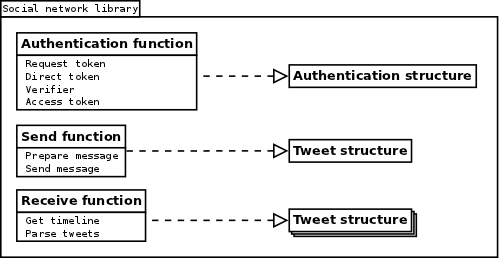
\includegraphics[scale=0.75]{images/functional_design.png}
  \caption{Functional diagram representing the implemented design}
\end{figure}


\clearpage